% Sidst opdateret: 13/1 1994
\chapter{Optimering af kemiske netv{\ae}rk}
\label{clarke}
Teorien om kemiske netv{\ae}rk er udviklet af Clarke
[\citen{clarke}]. Hans netv{\ae}rksteori har v{\ae}ret
anvendt for at foretage ``optimeringer'' af modeller for
oscillerende kemiske reaktioner. Vi vil i dette kapitel
f{\o}rst gennemg{\aa} dele af Clarkes teori for derefter at
diskutere disse ``optimeringer''.

\section{Teori}
Clarkes netv{\ae}rksteori fremstiller den makroskopiske
kemiske kinetik p{\aa} en mere abstrakt m{\aa}de i forhold
til vores fremstilling i kapitel~\ref{cha:Historie}. Denne
fremstilling giver mulighed for at analysere meget
komplekse reaktioner. Vores fremstilling i dette afsnit
ligger t{\ae}t op af \cite{clarke}. Vi har medtaget nogle
af Clarkes eksempler, men vi har valgt ogs{\aa} at
gennemregne disse.

\subsection{Basale begreber}
\label{clarke:basal}
Kemisk reaktionskinetik tager ofte udgangspunkt i
reaktionsmekanismen for en kemisk reaktion. Et netv{\ae}rk
er basalt set det samme. Et netv{\ae}rk best{\aa}r af $n$
stoffer, $c_1, \ldots, c_n$, $r$ reaktioner, $R_1, \ldots,
R_r$, en netto-st{\o}kiometrisk matrix, $\gmatrix{\nu}$, og
en hastighedsfunktion, $\vec{v}(\vec{c}, \vec{k})$, hvor
$\vec{k}$ er en vektor best{\aa}ende af
hastighedskonstanterne for de $r$ reaktioner. Kinetikken
for et kemiske netv{\ae}rk er givet ved et system af
s{\ae}dvanlige 1.\ ordens differentialligninger

\begin{equation}
\label{clarke:ODE}
\frac{d\vec{c}}{dt} = \gmatrix{\nu}\vec{v}(\vec{c}, \vec{k}).
\end{equation}

Det er rimeligt at kr{\ae}ve, at $[c_i] \ge 0$. Vi vil
ligeledes kr{\ae}ve, at $v_i(\vec{c}, \vec{k}) \ge 0$. Hvis
en reaktion b{\aa}de er fremadg{\aa}ende og
tilbageg{\aa}ende, deles reaktionen i to fremadg{\aa}ende
reaktioner. Det vil sige, at reaktionen $A
\rightleftharpoons B$ i netv{\ae}rksteorien vil blive
opfattet som de to reaktioner $A\rightarrow B$ og
$B\rightarrow A$.

\vspace{4.0mm}
Lad os illustrere disse begreber vha.\ Oregonatoren, som best{\aa}r af
f{\o}lgende reaktioner:

\begin{subequations}
\label{clarke:oregon}
\begin{eqalignno}
Y &\rightarrow X   \\
X + Y &\rightarrow \\
X & \rightarrow  2X + 2Z   \\
2X &\rightarrow   \\
2Z &\rightarrow fY  
\end{eqalignno}
\end{subequations}
hvor $X$ = \chem{HBrO_2}, $Y$ = \chem{Br^-} og $Z$ = \chem{Ce^{4+}}, og
reaktionshastigheder er givne ved 

\begin{subequations}
\begin{eqnarray}
v_1 &=& k_1[Y] \\
v_2 &=& k_2[X][Y] \\
v_3 &=& k_3[X] \\
v_4 &=& k_4[X]^2 \\
v_5 &=& k_5[Z]
\end{eqnarray}
\end{subequations}

Den st{\o}kiometriske matrix er

\[
\gmatrix{\nu} = \left(
\begin{array}{ccccc}
1 &-1& 1& -2& 0 \\
-1 & -1 & 0 & 0 & f \\
0 & 0 & 2 & 0 & -2 
\end{array} \right),
\]
mens koncentrationsvektoren er $\vec{c} = ([X], [Y], [Z])^T$, og
hastighedsvektoren er $\vec{v}(\vec{c}, \vec{k}) = (v_1, \ldots, v_5)^T$.

\subsection{St{\o}kiometriske b{\aa}nd}
I et netv{\ae}rk vil der ofte indg{\aa} st{\o}kiometriske
b{\aa}nd p{\aa} de involverede for\-bind\-elser. Naturlige
b{\aa}nd er grundstofbevarelse\footnote{I stedet for
grundstofbevarelse kunne der ogs{\aa} v{\ae}re tale om
bevarelse af funktionelle grupper.} og ladningsbevarelse.
Net\-v{\ae}rks\-teo\-rien tager hensyn til b{\aa}nd af
formen

\[
 \sum_i \gamma_{ki} [c_i] = C_k,
\]

hvor $\gamma_{ik}$ er passende konstanter og $C_k$ er den
totale koncentration af det $k$'te stof. Vi
kan skrive alle b{\aa}ndene p{\aa} matrixform

\[
  \gmatrix{\gamma}\vec{c} = \vec{C}.
\]

Matricen $\gmatrix{\gamma}$ kaldes for bevarelsesmatricen.
Ved at bruge de st{\o}kiometriske b{\aa}nd kan vi regne ud,
hvilke punkter i koncentrationsrummet, som fysisk er
meningsfulde. M{\ae}ngden af mulige koncentrationer
betegner vi med $\Pi_{\vec{c}}(\vec{C})$. Denne m{\ae}ngde
defineres ved

\begin{equation}
\Pi_{\vec{c}}(\vec{C}) \equiv \{\vec{c} | [c_i] \ge 0 \wedge
\gmatrix{\gamma}\vec{c} = \vec{C}\}.
\end{equation}

M{\ae}ngden vil ofte v{\ae}re konveks, dvs.\ det korteste
liniestykke, som forbinder to punkter i m{\ae}ngden, vil
selv v{\ae}re i m{\ae}ngden. Dimensionen af
$\Pi_{\vec{c}}(\vec{C})$ er $d$, eller sagt med andre ord:
Der er $d$ uafh{\ae}ngige dynamiske variable. Dimensionen
af $\Pi_{\vec{c}}(\vec{C})$ kan findes som rangen af
$\gmatrix{\nu}$. De resterende $n-d$ variable bestemmes af
de st{\o}kiometriske b{\aa}nd.

\vspace{4.0mm}
Vi ser p{\aa} et simpelt eksempel svarende til f{\o}lgende
to reaktioner

\begin{eqnarray*}
2 \chem{C} + \chem{O_2} &\rightarrow& 2 \chem{CO} \\ 
2 \chem{CO} + \chem{O_2} &\rightarrow& 2 \chem{CO_2}.
\end{eqnarray*}

Der er to naturlige b{\aa}nd; nemlig bevarelsen af
\chem{C}- og \chem{O}-atomer. B{\aa}ndene er

\begin{eqnarray*}
[{\chem{C}}] + [{\chem{CO}}] + [{\chem{CO_2}}] &=& C_{\chem{C}}, \\
2 [{\chem{O_2}}] + [{\chem{CO}}] + 2 [{\chem{CO_2}}] &=& C_{\chem{O}},
\end{eqnarray*}
og bevarelsesmatricen er

\[
\gmatrix{\gamma} = \left(
\begin{array}{ccc}
1 & 1 & 1 \\
2 & 1 & 2 
\end{array}\right).
\]

\subsection{Str{\o}mme}
\label{clarke:EC}
Vi vil nu se p{\aa} station{\ae}re tilstande for et kemisk
netv{\ae}rk. En station{\ae}r l{\o}sning til ligning
\ref{clarke:ODE} er en vektor $\vec{c}(t)$, som opfylder
$\frac{d\vec{c}}{dt} = 0$. Men det betyder, at der findes
en hastighedsvektor $\vec{v}^0(\vec{c}, \vec{k})$, som
opfylder

\begin{equation}
\label{clarke:strom}
\gmatrix{\nu}\vec{v}^0(\vec{c}, \vec{k}) = 0.
\end{equation}

Ovenst{\aa}ende ligning kan siges at v{\ae}re den kemiske
analogi til Kirschhoffs regel i
el-l{\ae}re\footnote{Kirshhoffs regel siger, at summen af
str{\o}mmene hen mod en knude i et elektrisk netv{\ae}rk er
nul \cite[s.\ 656]{fysikA}. Reglen er en konsekvens af
loven om ladningsbevarelse, samt at et hvert kurveintegral
(ved en lukket kurve) over det elektriske felt er nul.}.
Derfor vil vi kalde hastigheden $\vec{v}^0$ for en
str{\o}m.

\vspace{4.0mm}
Str{\o}mmene vil udg{\o}re et rum, og det er derfor
naturligt at indf{\o}re et symbol for dette rum. Vi
v{\ae}lger $\varrho_{\vec{v}}$. Rummet er formelt defineret
som alle de str{\o}mme som opfylder ligning
\ref{clarke:strom}, eller

\begin{equation}
\varrho_{\vec{v}} \equiv \{ \vec{v}^0 \in \overline{\R}^r_+ |
\gmatrix{\nu}\vec{v}^0 (\vec{c}, \vec{k}) = 0 \}.
\end{equation}

Denne m{\ae}ngde kaldes for {\em str{\o}mkeglen}. Hvis der
l{\ae}gges et snit (et hyperplan, som sk{\ae}rer akserne i
koncentrationsrummet) gennem str{\o}mkeglen, vil der
fremkomme en polytop. Det er muligt at vise, at
str{\o}mkeglen ogs{\aa} kan repr{\ae}senteres ved

\begin{equation}
\varrho_{\vec{v}} = \{ \matrix{E}\vec{j} | \vec{j} \in
\overline{\R}^f_+\}.
\end{equation}

S{\o}jlerne i $\matrix{E}$ er en basis for nulrummet til
hastighedsrummet. Det er mulig at vise, at str{\o}mkeglen
kan skrives som

\begin{subequations}
  \begin{equation}
    \varrho_{\vec{v}} = \{ \lambda\vec{v}^0 | \vec{v}^0\in
    \Pi_{\vec{v}},\lambda \ge 0\},
  \end{equation}

  \begin{equation}
    \Pi_{\vec{v}} \equiv \{\vec{v}^0\in \overline{\R}^r_ |
    \gmatrix{\nu}\vec{v}^0 = 0,\vec{e}_r^t\vec{v}^0 = \matrix{I} \}.
  \end{equation}
\end{subequations}

M{\ae}ngden $\Pi_{\vec{v}}$ kaldes for str{\o}mpolytopen.
Vi er i stand til at omskrive $\Pi_{\vec{v}}$ til

\begin{equation}
  \Pi_{\vec{v}} = \{ \matrix{E}\vec{j} | \vec{j}\in\overline{\R}^f_+,
  \vec{e}_f^t\vec{j} = \matrix{I} \},
\end{equation}

hvor vektoren $\vec{e}_f^t$ best{\aa}r af $f$ 1-taller.
Dimensionen af $\Pi_{\vec{v}}$ er $r-d-1$. S{\o}jlerne i
matricen $\matrix{E}$ danner siderne i str{\o}mkeglen, og
de kaldes for {\em ekstreme str{\o}mme}. Dimensionen af
denne basis er $f$. Selvom de ekstreme str{\o}mme danner en
basis for nulrummet, er det ikke alle baser, der kan
bruges. F.eks.\ vil baser, hvori der indg{\aa}r negative
elementer, ikke kunne bruges\footnote{Metoden i
\cite{Mat1LA}, som er den mest almindelige i line{\ae}r
algebra, kan generelt ikke bruges, da den ikke sikrer, at
elementerne er ikke-negative.}, da vi ikke {\o}nsker
negative reaktionshastigheder. De ekstreme str{\o}mme kan
findes ved at l{\o}se ligningssystemet

\begin{equation}
\matrix{B}\vec{v}^0 = \vec{b},
\end{equation}
hvor 

\[
\matrix{B} = \left[
\begin{array}{c}
\gmatrix{\nu} \\
1 \cdots 1 
\end{array} \right]
\]

og $\vec{b} = (0, \cdots, 0, 1)^T$. Rangen af $\matrix{B}$
er $d+1$, da der i $\matrix{B}$ er indf{\o}rt en line{\ae}r
uafh{\ae}ngig r{\ae}kke. Vi kan v{\ae}lge $d+1$ s{\o}jler
fra $\matrix{B}$ og p{\aa} den m{\aa}de konstruere en
kvadratisk matrix. Udv{\ae}lges samtidig de
sammenh{\o}rende elementer i $\vec{b}$, kan vi udregne
elementer i $\vec{v}^0$. Ikke alle de fremkomne
ligningssystemer vil have en acceptabel l{\o}sning
(ikke-negative elementer i $\vec{v}^0$). Men ved at
pr{\o}ve alle kombinationerne af s{\o}jler i $\matrix{B}$,
er vi i stand til at finde alle de ekstreme str{\o}mme.

\vspace{4.0mm}
Lad os i detaljer finde de ekstreme str{\o}mme til
Oregonatoren, som er defineret i (\ref{clarke:oregon}).
Rangen ($d$) af $\gmatrix{\nu}$ er 3. Derved bliver $\dim
\Pi_v = 1$. Vi skal v{\ae}lge fire s{\o}jler ud fra
$\gmatrix{\nu}$. Det kan g{\o}res p{\aa} fem m{\aa}der.

\begin{enumerate}
  \item
    \begin{equation}
      \left( 
      \begin{array}{cccc}
        -1 & 1 & -2 & 0 \\
        -1 & 0 & 0  & 1 \\
         0 & 2 & 0  & -2 \\
         1 & 1 & 1  & 1 
       \end{array}
       \right) \cdot
       \left(
       \begin{array}{c}
         v_2 \\
         v_3 \\
         v_4 \\
         v_5
       \end{array}
       \right) = 
       \left(
       \begin{array}{c}
         0 \\
         0 \\
         0 \\
         1
       \end{array}
       \right) 
     \end{equation}
     
     Dette svarer til de fire ligninge
     \begin{eqnarray*}
       -v_2 + v_3 -2 v_4 &=& 0 \\
       -v_2 + v_5        &=& 0 \\
       2v_3 - 2v_4       &=& 0 \\
       v_2 +v_3 +v_4 +v_5 &=& 1 
     \end{eqnarray*}
     
     Vi ser umiddelbart tre relationer, som skal v{\ae}re opfyldt

     \begin{eqnarray*}
       v_3 &=& v_4 \\
       v_2 &=& v_5 \\
       -v_2-v_3 &=& 0
     \end{eqnarray*}

     Der g{\ae}lder med andre ord $v_2 = -v_3$, og normeringen  
     medf{\o}rer ligningen $v_2-v_2-v_2+v_2 = 1$, hvilket er umuligt.
   \item
     \begin{equation}
       \left(
       \begin{array}{cccc}
         1 & 1 & -2 & 0 \\
         -1 & 0 & 0 & 1 \\
         0 & 2 & 0 & -2 \\
         1 & 1 & 1 & 1
       \end{array}
       \right) \cdot
       \left(
       \begin{array}{c}
         v_1 \\
         v_3 \\
         v_4 \\
         v_5
       \end{array}
       \right) =
       \left(
       \begin{array}{c}
         0 \\
         0 \\
         0 \\
         1
       \end{array}
       \right).
     \end{equation}
     
     Der kommer fire ligninger ud af denne matrixmultiplikation
     
     \begin{eqnarray*}
       v_1 + v_3 - 2v_4 &=& 0 \\
       -v_1 + v_5 &=& 0 \\
       2v_3 - 2v_5 &=& 0 \\
       v_1 + v_3 + v_4 + v_5 &=& 1
     \end{eqnarray*}
     
     Det ses let, at $v_1=v_3=v_4=v_5$, og ved normeringen f{\aa}s
     derfor $v_1=v_3=v_4=v_5 = \frac{1}{4}$.

   \item
     \begin{equation}
       \left(
       \begin{array}{cccc}
         1 & -1 & -2 & 0 \\
         -1 & -1 & 0 & 1 \\
         0 & 0 & 0 & -2 \\
         1 & 1 & 1 & 1
       \end{array}
       \right) \cdot
       \left(
       \begin{array}{c}
         v_1 \\
         v_2 \\
         v_4 \\
         v_5
       \end{array}
       \right) = 
       \left(
       \begin{array}{c}
         0 \\
         0 \\
         0 \\
         1
       \end{array}
       \right).
     \end{equation}

     F{\o}rst f{\aa}r vi fire ligninger
     
     \begin{eqnarray*}
       v_1 - v_2 - 2v_4 &=& 0 \\
       -v_1 - v_2 + v_5 &=& 0 \\
       -2v_5 &=& 0 \\
       v_1 + v_2 + v_4 + v_5 &=& 1 
     \end{eqnarray*}

     Fra den anden ligning har vi, at $v_1 = -v_2$, mens vi fra den f{\o}rste
     har $v_1 = v_4$. Men da hastighederne ikke m{\aa} v{\ae}re
     negative, s{\aa} m{\aa} der g{\ae}lde $v_1 = v_2 = 0$. Den sidste
     ligning giver os (vha.\ resultaterne fra de tre f{\o}rste) $v_1
     =1$. Det er i modstrid med tidligere resultater og er derfor
     ikke muligt.
   \item
     \begin{equation}
       \left(
       \begin{array}{cccc}
         1 & -1 & 1 & 0 \\
         -1 & -1 & 0 & 1 \\
         0 & 0 & 2 & -2 \\
         1 & 1 & 1 & 1
       \end{array}
       \right) \cdot
       \left(
       \begin{array}{c}
         v_1 \\
         v_2 \\
         v_3 \\
         v_5
       \end{array}
       \right) = 
       \left(
       \begin{array}{c}
         0 \\
         0 \\
         0 \\
         1
       \end{array}
       \right).
     \end{equation}
     
     De fire ligninger, som fremkommer ved multiplikationen, er
     
     \begin{eqnarray*}
       v_1 - v_2 + v_3 &=& 0 \\
       -v_1 - v_2 + v_5 &=& 0 \\
       2v_3 - 2v_5 &=& 0 \\
       v_1 + v_2 + v_3 + v_5 &=& 1
     \end{eqnarray*}
       
     Fra de tre f{\o}rste f{\aa}r vi $v_1 = 0$ og $v_2 = v_3 = v_5$.
     De sidste ligning giver os, at $v_2 = v_3 = v_5 =
     \frac{1}{3}$. 
   \item
     \begin{equation}
       \left(
       \begin{array}{cccc}
         1 & -1 & 1 & -2 \\
         -1 & -1 & 0 & 0 \\
         0 & 0 & 2 & 0 \\
         1 & 1 & 1 & 1 
       \end{array}
       \right) \cdot
       \left(
       \begin{array}{c}
         v_1 \\
         v_2 \\
         v_3 \\
         v_5 \\
       \end{array}
       \right) = 
       \left(
       \begin{array}{c}
         0 \\
         0 \\
         0 \\
         1 
       \end{array}
       \right).
     \end{equation}
       
     Matrixmultiplikationen giver os f{\o}lgende fire ligninger

     \begin{eqnarray*}
       v_1 - v_2 + v_3 -2v_4 &=& 0 \\
       -v_1 - v_2 &=& 0 \\
       2v_3 &=& 0 \\
       v_1 + v_2 + v_3 + v_4 &=& 1 
     \end{eqnarray*}
     
     De tre f{\o}rste ligninger medf{\o}rer $v_1 = v_2 = v_3 = v_4 =
     0$, og derved kan den sidste ligning ikke l{\o}ses.
\end{enumerate}

Der er alts{\aa} kun to ekstreme str{\o}mme i Oregonatoren.
Str{\o}mkeglens basis er med andre ord

\begin{equation}
\matrix{E} = \left(
\begin{array}{cc}
0 & 1 \\
1 & 0 \\
1 & 1 \\
0 & 1 \\
1 & 1
\end{array}
\right).
\end{equation}

Der findes en udgave af Oregonatoren, som kaldes {\em Split
Oregonatoren} [\citen{tina1}]. Den er defineret ved
f{\o}lgende seks reaktioner

\begin{eqnarray*}
\chem{BrO_3^-} + \chem{Br^-} &\rightarrow& \chem{HBrO_2} \\
\chem{HBrO_2} + \chem{Br^-} &\rightarrow& \chem{P} \\
\chem{BrO_3^-} + \chem{HBrO_2} &\rightarrow& 2\chem{HBrO_2} +
2\chem{Ce^{4+}} \\
2\chem{HBrO_2} &\rightarrow& \chem{P} \\
\chem{Ce^{4+}} + \chem{BrMA} &\rightarrow& \chem{Br^-} \\
\chem{Ce^{4+}} + \chem{MA} &\rightarrow& \chem{P} \\
\end{eqnarray*}

hvor \chem{P} er en inaktivt produkt. Der er tale om et
netv{\ae}rk, som er {\ae}kvivalent til Oregonatoren, men
reaktionen, hvor den st{\o}kiometriske parameter $f$
indg{\aa}r, er blevet delt (heraf navnet) i to reaktioner.
Dette netv{\ae}rk har fire ekstreme str{\o}mme. Vi vil ikke
gennemg{\aa} detajlerne i udregningerne. De
ikke-normaliserede ekstremme str{\o}mme er

\begin{equation}
\matrix{E} = \left(
\begin{array}{cccc}
0 & 0 & 1 & 4 \\
0 & 1 & 3 & 0 \\
2 & 1 & 2 & 2 \\
1 & 0 & 0 & 3 \\
0 & 1 & 4 & 4 \\
4 & 1 & 0 & 0 \\
\end{array}
\right).
\end{equation}

\noindent
Figur \ref{clarke:SplitEC} viser, hvordan de ekstreme
str{\o}mme danner en str{\o}mkegle. Figuren er et falsum,
da rummet hvor keglen er placeret, har dimensionen seks.

\boxfigure{t}{\textwidth}
{
\vspace{5.0mm}
\psfig{file=splitec.ps,height=5cm,width=13cm}
}
{
\caption{\protect\capsize
Str{\o}mkeglen for Split Oregonatoren. Der er fire ekstreme str{\o}mme i
de 6-dimensionale hastighedsrum. Str{\o}mkeglen er besk{\aa}ret af et
hyperplan, s{\aa} der fremkommer en polytop. Tegningen er fra
\protect\cite{tina1}.
\label{clarke:SplitEC}}
}

\section{Optimering af modeller}
Clarkes netv{\ae}rksteori g{\o}r det muligt at foretage en
optimering af en model. Optimering betyder her, at
hastighedskonstanterne v{\ae}lges, s{\aa} modellen passer
bedst muligt med eksperimenterne
[\citen{tina1,tina2,Prag:tina,Prag:Hynne}].

\vspace{4.0mm}
Det er muligt at benytte kontinueringsmetoder til at
optimere en parameter, f.eks.\ en hastighedskonstant
[\citen{Prag:Kubicek}]. Men det har vist sig, at
kontinueringsteknikker ikke altid giver de bedste
resultater [\citen{HopfQuench}]. Problemet er, at de ikke
unders{\o}ger hele parameterrummet, men kun en delm{\ae}ngde
heraf.

\vspace{4.0mm}
Det er generelt et problem at finde hastigshedskonstanterne
for komplekse reaktionssystemer eksperimentelt. I mange af
reaktionerne vil der indg{\aa}r stoffer, som enten har
meget korte levetider eller er til stede i s{\aa} sm{\aa}
koncentrationer, at det umuligt at m{\aa}le dem. Der kan
opstilles fem krav til det optimerende netv{\ae}rk.

\begin{enumerate}
  \item
    Det station{\ae}re punkt skal v{\ae}re lig det eksperimentelt fundne.
  \item
    Punktet i parameterrummet skal v{\ae}re en Hopfbifurkation.
  \item
    Frekvensen for oscillationerne skal stemme overens med
    eksperimenterne.
  \item
    Egenv{\ae}rdierne for Jacobimatricen skal passe med de eksperimentelt
    beregnede egenv{\ae}rdier.
  \item
    Alle eksperimentelt kendte koncentrationer skal kunne
    godtg{\o}res af modellen.
\end{enumerate}

\subsection{Baggrunden}
Ved en superkritisk Hopfbifurkation g{\aa}r systemet fra et
ustabilt station{\ae}rt punkt til en stabil
gr{\ae}nsecyklus. Kapitel~\ref{cha:Quench} beskriver en
succesrig eksperimentel metode i dette tilf{\ae}lde.
Metoden bestemmer egenvektorerne til Jacobimatricen i
bifurkationspunktet.

\vspace{4.0mm}
Fra quenchingeksperimenter kender vi venstre- og
h{\o}jreegenvektorerne til Jacobimatricen

\begin{eqnarray*}
\matrix{J}\vec{e}_- &=& i\omega \vec{e}_- \\
\vec{e}^-\matrix{J} &=& i\omega\vec{e}^-.
\end{eqnarray*}
De kinetiske ligninger er (potenslov kinetik er her antaget)

\[
\frac{dc_p}{dt} = \sum_r \nu_{pr}k_r\prod_s c_s^{\kappa_{sr}}.
\]

Vi kan derfor finde et udtryk for Jacobimatricen ved at
differentiere med hensyn til $c_s$. G{\o}res dette, f{\aa}r
vi

\begin{equation}
J_{ps} = \sum_r \nu_{pr}\kappa_{sr}\frac{v_r}{c_s},
\end{equation}

idet $v_r$ er hastigheden af den $r$'te reaktion. Vi kan
se, at hvis vi multiplicerer $\vec{v}$ med en positiv
konstant $\gamma_{\vec{v}}$ bliver $\matrix{J}$ ogs{\aa}
$\gamma_{\vec{v}}$ gange st{\o}rre. Egenvektorerne
forbliver de samme, men egenv{\ae}rdierne bliver alle
multipliceret med $\gamma_{\vec{v}}$.

\vspace{4.0mm}
Hvis vi multiplicerer koncentrationsvektoren med en
konstant, bliver egen\-v{\ae}r\- dien divideret med denne
konstant.

\vspace{4.0mm}
Vi ser, at n{\aa}r et punkt har en egenv{\ae}rdi som er
imagin{\ae}r, s{\aa} vil et hvert skaleret punkt ogs{\aa}
have det. Det betyder, at vi kan skalere frekvensen af
oscillationerne, s{\aa} den kommer til at stemme overens
med eksperimenterne. Med andre ord, s{\aa} er quechingdata
invariante ved en skalering. Det betyder, at s{\o}gningen i
str{\o}mkeglen kan reduceres til en s{\o}gning i en polytop
(et snit gennem keglen), hvorefter en skalering foretages,
s{\aa} den {\o}nskede frekvens opn{\aa}s. Det er vigtigt at
skalere b{\aa}de koncentrationer og hastighedskonstanter
samtidig, da vi ellers kunne komme i den situation, at det
nye punkt ikke l{\ae}ngere udgjorde et
Hopfbifurkationspunkt i parameterrummet.

\vspace{4.0mm}
Den f{\o}romtalte polytop er en konveks m{\ae}ngde. Derfor
kan alle punkter i polytopen skrives som en konveks
kombination, som i dette tilf{\ae}lde er

\[
  \vec{c} = \sum_i j_i E_i,
\]

hvor $j_i$ er positive reelle tal, som opfylder $\sum_i j_i
=1$.

\vspace{4.0mm}
N{\aa}r vi skal optimere et netv{\ae}rk, skal vi begynde med
at udregne de ekstreme str{\o}mme. Derved finder vi den
omtalte polytop. Vi skal derefter unders{\o}ge alle punkter
i polytopen, og n{\aa}r vi finder en Hopfbifurkation, kan vi
skalere frekvensen, s{\aa}ledes at den passer med den
eksperimentelle frekvens. Men s{\aa}dan s{\o}gning i
polytopen er kun mulig, hvis den nedbrydes i simple
geometriske figurer, f.eks.\ trekanter.

\subsection{En grafisk afpr{\o}vning}
\label{clarke:test}
Det er muligt at foretage en afpr{\o}vning af quenchingdata [\citen{tina2}].
Ideen er at bruge en simpel metode, som er i stand til at
afg{\o}re om et netv{\ae}rk er muligt, dvs.\ om
netv{\ae}rket kan forklare quenchingdata.

\vspace{4.0mm}
Den komplekse amplitude, $w_s$, for stof $s$ er givet ved

\begin{equation}
  w_s = a_se^{i\theta_s},
\end{equation}
mens den komplekse quenchingamplitude er

\begin{equation}
  f_s = -q_se^{i\phi_s},
\end{equation}

hvor $a_s$ er den egentlige amplitude, $\theta_s$ fasen,
$q_s$ er quenchingm{\ae}ngden og $\phi_s$ er quenchingfasen.
Ved en Hopfbifurkation g{\ae}lder der

\begin{subequations}
  \begin{equation}
    -i\omega w_p = \sum_s J_{ps} w_s,
  \end{equation}
  
  \begin{equation}
    -\frac{i\omega}{f_s} = \sum_s \frac{J_{ps}}{f_p},
  \end{equation}
\end{subequations}

hvor $\matrix{J}$ er Jacobimatricen. Disse to udtryk
omskrives til

\begin{subequations}
  \begin{equation}
    -iw_p = \sum_r L_{pr}\cdot\frac{v_r}{\omega},
  \end{equation}

  \begin{equation}
    \label{clarke:10b}
    -\frac{i}{f_s} = \sum_r R_{sr}\cdot\frac{v_r}{c_s\omega},
  \end{equation}
\end{subequations}

hvor $v_r$ er hastigheden af reaktion $r$. Elementerne i de
to matricer $\matrix{L}$ og $\matrix{R}$ er

\begin{subequations}
  \begin{equation}
    L_{pr} = \sum_s \frac{\nu_{pr}\kappa_{sr}w_s}{c_s},
  \end{equation}

  \begin{equation}
    R_{sr} = \sum_p \frac{\nu_{pr}\kappa_{sr}}{f_p}.
  \end{equation}
\end{subequations}

Elementerne i matricen $\matrix{R}$ kaldes for de komplekse
reaktionsamplituder. Ind\-f{\o}rer vi nu
$K_{sr}=\frac{v_r}{c_s\omega}$, kan vi omskrive
(\ref{clarke:10b}) til

\begin{equation}
  -\frac{i}{f_s} = \sum_r R_{sr}K_{sr},
\end{equation}

dvs.\ der er tale om en effektiv 1.\ ordens
hastighedskonstant. Vi kan med andre ord betragte
$-\frac{i}{f_s}$ som en linear kombination af vektorerne
$R_{s1}, \ldots, R_{sr}$ med koefficienterne $K_{s1},
\ldots, K_{sr}$, hvor $r$ er antallet af reaktioner. For at
dette skal v{\ae}re muligt, s{\aa} er det n{\o}dvendigt og
tilstr{\ae}kkeligt, at vektoren $-\frac{i}{f_s}$ ligger i den
sektor, som dannes i den spidse vinkel mellem $R_{sr}$ og
$R_{sr\prime}$ for alle $r$ og $r\prime$. Figur
\ref{clarke:GrafTest} skitserer dette i en model med tre
stoffer. Hvis ovenst{\aa}ende betingelse ikke er opfyldt, er
quenchingdata ikke kompatible med modellen, og
netv{\ae}rket er ikke i stand til at forklare
quenchingdata. Det betyder, at netv{\ae}rket m{\aa}
kasseres.

\boxfigure{t}{\textwidth}{
\begin{center}
 \setlength{\unitlength}{0.012500in}%
\begin{picture}(145,273)(65,510)
\thicklines
\put(120,720){\vector( 0,-1){200}}
\put(120,720){\vector(-1, 1){ 40}}
\put(120,720){\vector( 4, 3){ 31.200}}
\multiput(120,720)(7.82609,0.00000){12}{\line( 1, 0){  3.913}}
\put(210,720){\vector( 1, 0){0}}
\put(115,510){\makebox(0,0)[lb]{\smash{$R_{s1}$}}}
\put( 65,765){\makebox(0,0)[lb]{\smash{$R_{s2}$}}}
\put(150,750){\makebox(0,0)[lb]{\smash{$R_{s3}$}}}
\put(210,720){\makebox(0,0)[lb]{\smash{$-\frac{i}{f_s}$}}}
\end{picture}

 \vspace{5.0mm}
\end{center}
}
{
\caption{\protect\capsize
Grafisk afpr{\o}vning af quenchingdata, fra
\protect\cite{tina1}.}
\label{clarke:GrafTest}
}

\vspace{4.0mm}
Denne form for grafisk afpr{\o}vning vil v{\ae}re
n{\o}dvendig, n{\aa}r man foretager optimeringer. P{\aa}
den m{\aa}de er det muligt at se, om de optimerede
parametre er fysisk mulige og derved om modellen
overhovedet er rimelig.

\subsection{Eksempler}
Flere modeller er til dags dato allerede blevet optimeret
[\citen{tina2}]. Det drejer sig om to forskellige udgaver af
Oregonatoren. Optimeringerne udviser god overensstemmelse
med de eksperimentelle v{\ae}rdier.

\vspace{4.0mm}
En udvidet udgave af Oregonatoren, den s{\aa}kaldte {\em
Extended Oregonator}, har bl.a.\ v{\ae}ret anvendt ved
optimeringer. Denne udgave af Oregonatoren er defineret ved

\begin{subequations}
  \begin{eqnarray}
        &\rightarrow& \chem{BrO_3^-} \\
    \chem{BrO_3^-}+\chem{Br^-} &\rightarrow& \chem{HBrO_2}+\chem{HBrO} \\
    \chem{HBrO_2}+\chem{Br^-} &\rightarrow& 2\chem{HBrO} \\
    \chem{BrO_3^-}+\chem{BrO_2} &\rightleftharpoons& 2\chem{BrO_2} \\
    \chem{BrO_2}+\chem{BrO_2} &\rightleftharpoons&
    \chem{HBrO_2}+\chem{Ce^{4+}} \\
    \chem{Br^-}+\chem{HBrO} &\rightarrow& \chem{Br_2} \\
    \chem{Ce^{4+}}+\chem{CHBr(COOH)_2} &\rightarrow& \chem{Br^-} +\chem{Ce^{3+}} \\
    \chem{Ce^{4+}}+\chem{CH_2(COOH)_2} &\rightarrow& \chem{Ce^{3+}} \\
    \chem{HBrO}+\chem{CH_2(COOH)_2} &\rightarrow& \chem{Br^-} \\
    \chem{HBrO}+\chem{CH_2(COOH)_2} &\rightarrow& \chem{CHBr(COOH)_2} \\
    \chem{Br_2}+\chem{CH_2(COOH)_2} &\rightarrow& \chem{Br^-}+\chem{CHBr(COOH)_2}
  \end{eqnarray}
\end{subequations}

\newpage
For denne model har vi f{\o}lgende tabel

\vspace{0.5cm}
\begin{center}
\begin{tabular}[h]{l|rr|rr}
\hline
Stof & 
\multicolumn{2}{c|}{Optimerede} & \multicolumn{2}{c}{Eksperimentelle} \\
 & amplituder & vinkler & amplituder & vinkler \\ \hline
\chem{HBrO_2} & 0.24 & 94   & 0.20  & 92   \\
\chem{HBrO}   & 1.57 & -118 & 1.58  & -120 \\
\chem{Br_2}   & 0.28 & -104 & 0.093 & -103 \\
\chem{Br^-}   & 0.28 & -101 & 0.11  & -104 \\
\chem{Ce^{4+}} & 0.89 & -135 & 0.43  & -128 \\ \hline
\end{tabular}
\end{center}

Optimeringerne er sket for at finde optimale
hastighedskonstanter. For den udvidede Oregonator finder M{\o}ller
{\em et al.} f{\o}lgende

\begin{center}
\begin{tabular}{crr}
Reaktion & Optimerede           & Litteratur \\ \hline
0        & $3.39\cdot 10^{-5}$  & $3.39\cdot 10^{-5}$ \\
1        & $30$                 & $2$ \\
2        & $7.4\cdot 10^6$      & $3\cdot 10^6$ \\
3        & $117$                & $42$ \\
4        & $9.0\cdot 10^4$      & $8\cdot 10^4$ \\
5        & $2.0\cdot 10^6$      & $3\cdot 10^9$ \\
6        & $48$                 & $30$ \\
7        & $1.7$                & $0.10$ \\
8        & $0.99$               & ingen litteraturv{\ae}rdi \\
9        & $2.7$                & $8.2$ \\
10       & $23$                 & $40$ \\
-3       & $5.9\cdot 10^7$      & $4.2\cdot 10^7$ \\
-4       & $2.0\cdot 10^4$      & $8.4\cdot 10^3$ \\ \hline
\end{tabular}
\end{center}

\noindent
idet negative reaktionsnumre refererer til de
tilbageg{\aa}ende reaktioner. Det interessante er, at det
er muligt at finde en hastighedskonstant, som ikke kan
findes i litteraturen. Det har stor betydning ved de videre
numeriske studier af modellen. Netv{\ae}rket passerer den
grafiske afpr{\o}vning.

\vspace{4.0mm}
Nedenst{\aa}ende tabel viser resultaterne af en optimering
af en anden udgave af Oregonatoren, {\em Split
Orogonatoren} (amplituder er angivet i enheder af
\chem{Ce^{4+}}-amplituden, mens vinkler er angivet i
grader).

\vspace{0.5cm}
\begin{center}
\begin{tabular}[h]{l|rr|rr}
\hline
Stof & 
\multicolumn{2}{c|}{Optimerede} & \multicolumn{2}{c}{Eksperimentelle} \\
 & amplituder & vinkler & amplituder & vinkler \\ \hline
\chem{HBrO_2} & 0.21 & 93 & 0.20 & 92 \\
\chem{Br^-}   & 0.22 & -97 & 0.11 & -104 \\
\chem{Ce^{4+}} & 0.56 & -121 & 0.43 & -128 \\ \hline
\end{tabular}
\end{center}

\noindent
Frekvensen for b{\aa}de de eksperimentelle og optimerede
data er 0.20 ${\rm s}^{-1}$. Metoden, som er omtalt i dette
kapitel, viser tydeligt, at de beregnede quenchingdata
stemmer ganske godt overens med de eksperimentelle data.
Som ved den udvidede Oregonator, var det
hastighedskonstanterne som skulle optimeres.
Nedenst{\aa}ende tabel viser resultaterne.

\begin{center}
\begin{tabular}{crr}
Reaktion & Optimerede      & Litteratur \\ \hline
1        & $4.0$           & $2$ \\
2        & $4.2\cdot 10^5$ & $3.2\cdot 10^6$ \\
3        & $101$           & $42$ \\
4        & $2.0\cdot 10^4$ & $3\cdot 10^3$ \\
5        & $40$            & $30$ \\
6        & $1.4$           & $0.10$ \\ \hline
\end{tabular}
\end{center}

Det viser sig, at Split Oregonatoren ikke er i stand til at
passere den grafiske afpr{\o}vning, som blev gennemg{\aa}et
i afsnit \ref{clarke:test}. Det betyder, at de optimerede
hastighedskonstanter ikke stemmer overens med
virkeligheden.
